% Example on how to use the Fonetik LaTeX2e class
\documentclass{fonetik}

% These are optional packages if you like:
% - nice fonts and symbols for mathematics
\usepackage{amsmath,amsfonts,latexsym,amssymb}
% - Unicode input encoding
\usepackage[utf8]{inputenc}
%\usepackage[T1]{fontenc}
% - language specific definitions (if not English)
%\usepackage[english]{babel}
% - extends the tabular syntax for tables.
\usepackage{array}
% - to insert nice eps figures
\usepackage{graphicx}

% defining hyphenation for difficult words is also optional
\hyphenation{si-mu-la-tion re-so-nance mo-dels}

% here you can also define some commands that you want to use
% later to simplify typing text
\newcommand{\BibTeX}{{\rm B\kern-.05em{\sc i\kern-.025em b}\kern-.08em
    T\kern-.1667em\lower.7ex\hbox{E}\kern-.125emX}}

% Here is the title, author and abstract definition
% Note:
% 1) affiliation should not specified if it is TMH
% 2) the abstract is defined in a nonstandard way
\title{An example on using the Fonetik \LaTeX2e class}
\author{Author Name$^1$, Author Name$^2$}
\affil{$^1$KTH Royal Institute of Technology,\\
  $^2$Department, University, Country\\
  \normalfont\texttt{author@kth.se, author@dept.uni.co}
}

\begin{document}
\maketitle

\begin{abstract}
This is an example on how to use the \LaTeX2e class {\tt
  fonetik.cls} for writing articles in the style adopted by the Fonetik
conference in Sweden. This example will describe some of the standard features
of \LaTeX2e and the additional commands provided by the class.
\end{abstract}

% note that LaTeX allows you to define cross references, but this is
% useless in here because there is no section numbering in the Fonetik
% style (unfortunately).
\section{Introduction}
Provided that you have the \verb|fonetik.cls| file in the same directory
as the \verb|.tex| file, or somewhere in the \LaTeX\ search path, the
document class is specified by the command:
\begin{verbatim}
\documentclass{fonetik}
\end{verbatim}

A number of packages can then be included depending of the special
needs of the author. This is done with the \verb|\usepackage| command
(look at the \verb|.tex| file in the distribution for examples).

The class disables headers, footers and page numbers, as defined by the
Fonetik recommendations. Please do not use footnotes in your test.

Title and author are defined as usual by the \verb|\title| and
\verb|\author| commands. A new command \verb|\affil| from the package
\verb|affil-it| is provided for affiliation. The abstract is defined using
the environment \verb|abstract| after the \verb|\begin{document}|
command.

Sections, subsections\ldots, are started with the usual
\verb|\section|, \verb|\subsection|\ldots\ commands. Section numbering is
disabled according to Fonetik recommendations.

For the rest, normal \LaTeX\ commands can be used to produce cross
references (\verb|\label| and \verb|\ref|), tables and figures, with
the corresponding environments, mathematical formulas, citations
(using the \verb|natbib| package that is automatically loaded by the
class). Note that setting labels to sections and subsections is
useless as there is no numbering in the Fonetik style
(unfortunately). Examples of this and more can be found in the rest of
this document. In case you are reading a PDF version of it
you are referred to the \verb|example.tex| file that was used to
generate them.

One of the best ways to produce a bibliography is to create a \BibTeX\
file (see \verb|example.bib| in the distribution). The citations can be
obtained by using one of the following commands. If the citation comes
in the end of a phrase, the \verb|\citep| command should be used,
e.g.
\begin{quote}
\ldots{}the first attempts to simulate the flow-induced oscillations
were based on a lumped- element model \citep{SmartAndSmarter68}.
\end{quote}
 If the author is cited directly in the text,
then the \verb|\citet| command should be used instead, e.g.
\begin{quote}
An essential improvement to the one-mass model was proposed by
\citet{DullAndMean98}, with their two-mass model.
\end{quote}
Because we are using unicode, you can write accented letters directly in your bib file as in \citep{accented}.
For more information, refer to the \BibTeX\ and {\tt natbib}
documentation \citep[e.g.][ch. 13]{companion}. Another good reference for
\LaTeX\ in general is \citep{short} (just google on the net).

\section{Inserting Figures and Tables}
Also the figures and tables can be inserted with standard \LaTeX\ 
commands. This is an example:
\begin{verbatim}
\begin{figure}
\centering
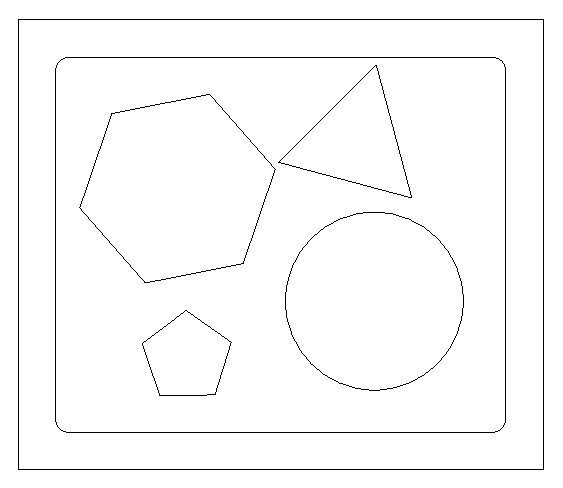
\includegraphics
  [width=\columnwidth]
  {figures/figb.eps}
\caption{An abstract figure.}
\label{fig:abstract}
\end{figure}
\end{verbatim}
The above code is used to produce Figure~\ref{fig:abstract}. Note that
I used the command \verb|\ref{fig:abstract}| to generate the figure
number in the previous sentence.
\begin{figure}
\center
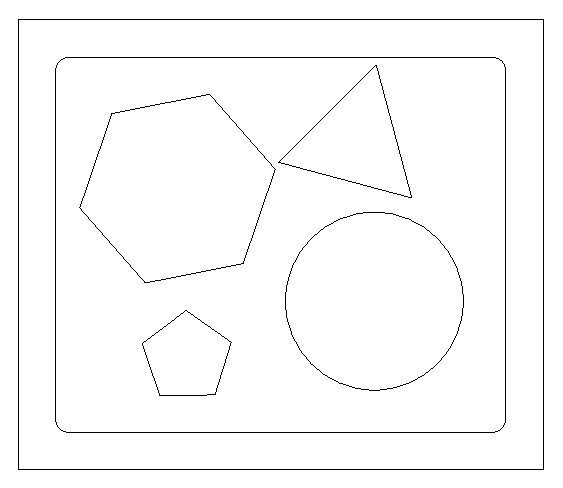
\includegraphics[width=\columnwidth]{figures/figb.eps}
\caption{A single column figure.}\label{fig:abstract}
\end{figure}

If you want to include figures that span two columns, use the
``starred'' version of the {\tt figure} environment, i.e.
\begin{verbatim}
\begin{figure*}
...
\end{figure*}
\end{verbatim}
An example will be given later.

Inserting tables is as easy, just remember to put the caption above the
table, i.e
\begin{verbatim}
\begin{table}[b]
\centering
\caption{This is the table
   caption (above the table)}
\label{tab:example}
\begin{tabular}{cc}
  \hline \hline
  Parameter & Value \\
  \hline
  \\
  $m$ & $0.00017$ $kg$   \\
  $L$ & $0.014$ $m$ \\
  $x_0$ & $0.005-0.1$ $mm$ \\
  \hline \hline
\end{tabular}
\end{table}
\end{verbatim}

\begin{table}[b]
\centering
\caption{This is the table caption
  (above the table)}
\label{tab:example}
\begin{tabular}{cc}
  \hline \hline
     Parameter & Value \\
     \hline
     \\
      $m$ & $0.00017$ $kg$   \\
      $L$ & $0.014$ $m$ \\
      $x_0$ & $0.005-0.1$ $mm$ \\
      \hline \hline
\end{tabular}
\end{table}

\begin{figure*}[!t]
\centering

\includegraphics[width=\textwidth]{figures/figa.eps}
\caption{A two-column figure.} \label{fig:concrete}
\end{figure*}

The above code is used to generate Table~\ref{tab:example}. Note that in this
case I added the option {\tt [b]} that indicates I wish the table to
be at the bottom of the page, if possible. Other options for floating
object placement are: {\tt [h]} for ``here'', i.e. the insertion point
in the text, {\tt [t]} for ``top'' that is the default, and {\tt [p]}
to put it in a special page that collects all floating objects. These
options are just an indication of preference, and they are overridden
by other type-setting rules. If you want to strengthen your
determination against the evil computerised type-setter, put an
exclamation mark in front of the option (\verb|[!h]|), but note that
the type-setter is still setting the rules, to some extent.

\subsection{Lots of meaningful words}
This section is just a filler to come to the next page.

Filler filler filler filler filler filler filler filler filler
filler filler filler filler filler filler filler filler filler
filler filler filler filler filler filler filler filler filler
filler filler filler filler filler filler filler filler filler

Filler filler filler filler filler filler filler filler filler
filler filler filler filler filler filler filler filler filler
filler filler filler filler filler filler filler filler filler
filler filler filler filler filler filler filler filler filler

Filler filler filler filler filler filler filler filler filler
filler filler filler filler filler filler filler filler filler
filler filler filler filler filler filler filler filler filler
filler filler filler filler filler filler filler filler filler

\subsection{It's never enough!}
Filler filler filler filler filler filler filler filler filler
filler filler filler filler filler filler filler filler filler
filler filler filler filler filler filler filler filler filler
filler filler filler filler filler filler filler filler filler

Filler filler filler filler filler filler filler filler filler
filler filler filler filler filler filler filler filler filler
filler filler filler filler filler filler filler filler filler
filler filler filler filler filler filler filler filler filler

Filler filler filler filler filler filler filler filler filler
filler filler filler filler filler filler filler filler filler
filler filler filler filler filler filler filler filler filler
filler filler filler filler filler filler filler filler filler

\section{A last example}
As promised in a previous section an example of a
two-column figure is Figure~\ref{fig:concrete}

\section{Acknowledgement}
The author is grateful to all the nice people using \LaTeX\ to typeset
their contribution to the QPSR. This work has been supported by lots
of patience and a whole load of irresponsibility.


\bibliographystyle{fonetik}
\bibliography{example}

\end{document}
